\documentclass[a4paper]{jsarticle}
\usepackage[dvipdfmx]{graphicx}
\usepackage{enumitem}

\setlist[enumerate,1]{label= \textcircled{\scriptsize \arabic*}}
\setlist[enumerate,2]{label= \arabic*.}

%% Hyphenation setting
\hyphenpenalty=1000\relax
\exhyphenpenalty=1000\relax
\sloppy

\begin{document}
% ------------------------------------------------------
% front cover
% ------------------------------------------------------

\large
\vspace{-5.0cm}
\hspace{-1.0cm}
情報工学実験II

\hspace{-1.0cm}
2019年5月8日

\Huge
\vspace{1.0cm}
\begin{center}
  食堂システム 要件定義書
\end{center}

\vspace{0.5cm}
\begin{center}
  \LARGE
  明石工業高等専門学校
\end{center}

\LARGE
\begin{center}
  \begin{tabular}{rl}
    E1507 & 泉 和哉 \\
    E1514 & 岡本 一真 \\
    E1533 & 西 総一朗
  \end{tabular}
\end{center}

\normalsize

\tableofcontents
\thispagestyle{empty}
\clearpage
\setcounter{page}{1}

% ------------------------------------------------------
% text start
% ------------------------------------------------------

\section{目的}
弊校には食堂がある。  食堂にはカレーなどの常設メニューと日替わりで提供されるメニューがあり、それぞれ格安で提供されるため、多くの学生に利用してもらっている。

しかし、「目当てのメニューが売り切れているかどうかが実際に食堂に行ってみないとわからない」「メニューが美味しいのかどうかが判断しづらく、メニュー選びの際に尻込みしてしまう」「目当てのメニューがいつ提供されるかはメニュー表を見ないと把握できない」といった課題があり、それらは学生が気軽に食堂を利用するための障壁の1つとなっている。

本プロダクトではそれらの課題を解決し、学生により気軽に食堂を利用してもらうことを目的とする。

\section{機能要件}
本プロダクトで実装する主な機能を以下に示す。

\begin{itemize}
  \item 学生が日ごとに提供されるメニューの名前や値段などを閲覧でき、各メニューの売り切れ情報を各人で更新できるようにする
  \item 学生がメニューのレビューを行え、全学生は全てのレビュー情報を閲覧できるようにする
  \item 学生が日替わりメニューにおいてお気に入りを登録でき、登録した日替わりメニューが提供される日は事前に通知を受け取れるようにする
  \item 食堂の従業員は新規のメニューを追加でき、提供メニューの売り切れ情報を含む全てのメニュー情報を変更できるようにする
  \item 多言語に対応し、留学生も利用しやすいようにする
\end{itemize}

なお、メニューの売り切れ情報は日付が変わるときにリセットされ、メニューのレビュー・お気に入り登録は学生がログインをすることによって可能となる。

学生・食堂の従業員のログインにはGoogleアカウントを利用する。

\newpage

\section{データフローダイアグラム (DFD)}
プロダクト全体のDFDを図\ref{dfd}に示す。

\begin{figure}[htbp]
  \centering
  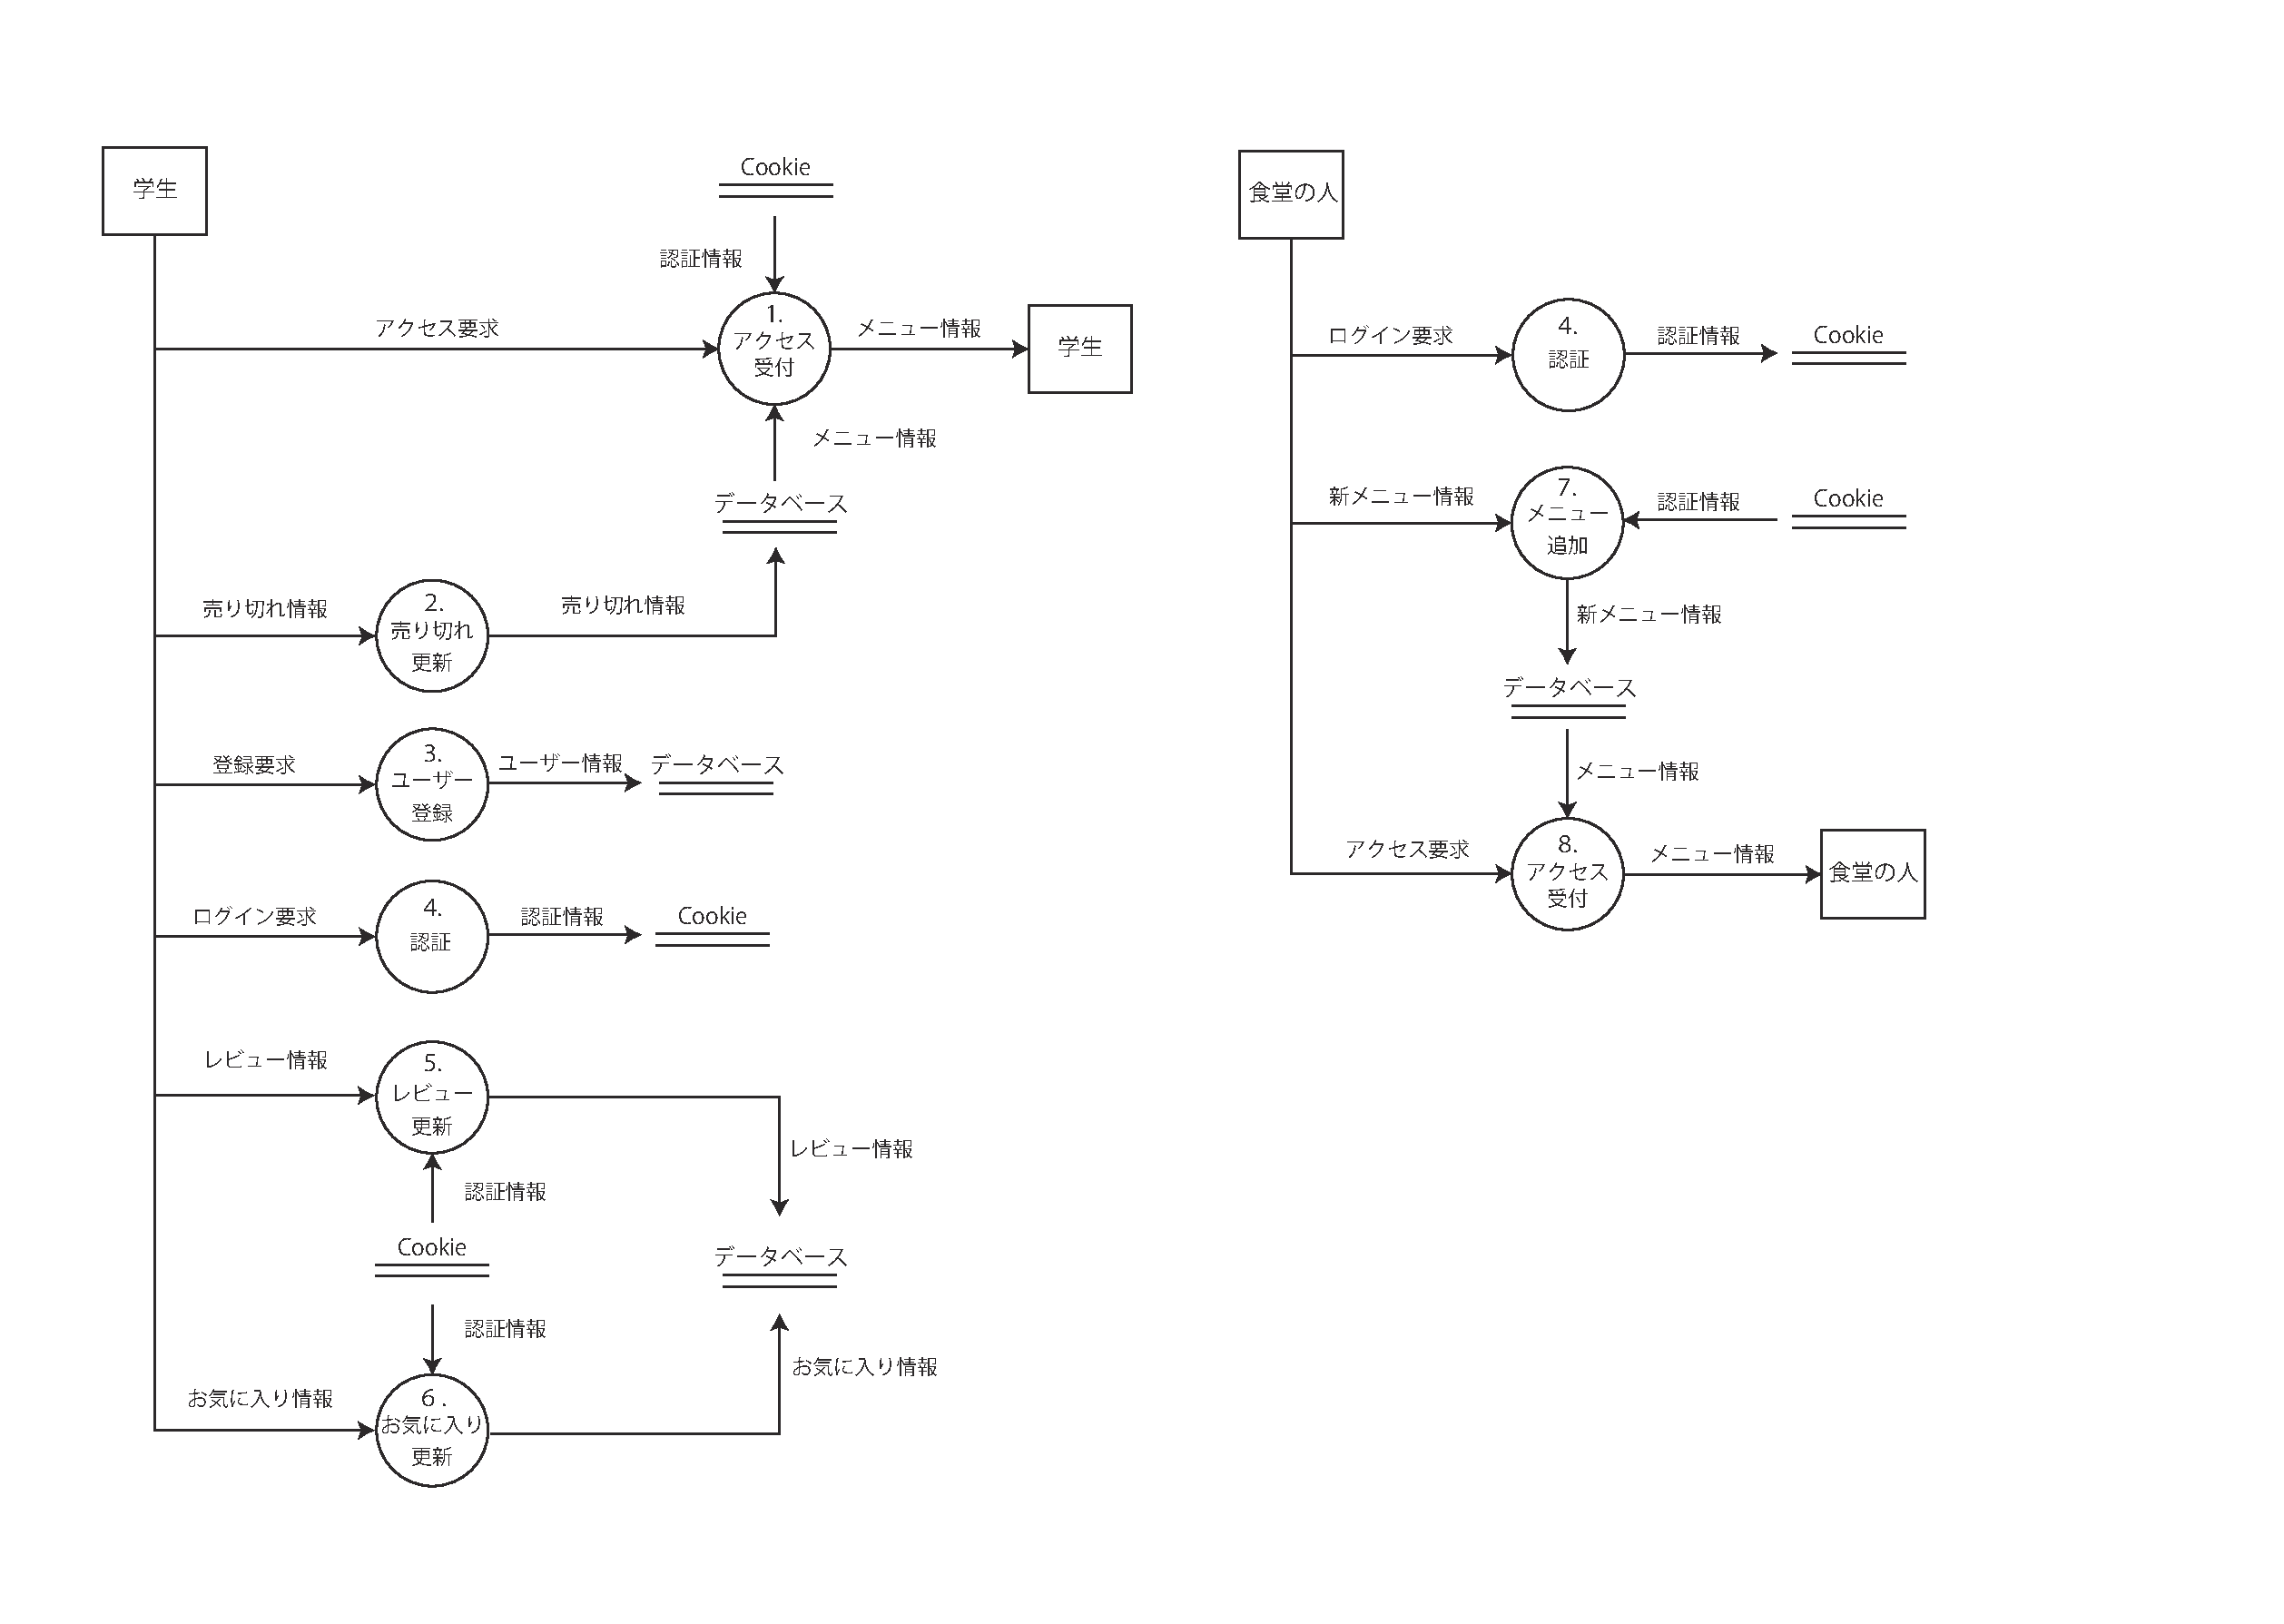
\includegraphics[scale=0.50]{DFD/DFD.pdf}
  \caption{DFD}
  \label{dfd}
\end{figure}

\newpage

\section{データディクショナリ}
図\ref{dfd}のDFDをもとに作成したデータディクショナリを以下に示す。

なお、「ID」、「○○ID」はそれぞれデータベース上での主キー、○○に対応するデータの外部キーを、 \\
「Google認証情報」はGoogleと連携してユーザログインを実現するために必要な情報を表す。

また、一度定義されたデータは、以降定義なしで使えるものとする。

\begin{enumerate}
  \item ファイル関連
  \begin{verbatim}
  データベース = {メニュー情報} + {日替わり提供情報} + {ユーザ情報} + {売り切れ情報}
    メニュー情報 = ID +品名+メニューのカテゴリ
                      +値段+エネルギー+脂質+タンパク質+ {レビュー情報}
      ID = 文字列
      品名 = 文字列
      メニューのカテゴリ = 文字列
      値段 = 整数
      エネルギー = 小数
      脂質 = 小数
      タンパク質 = 小数
      レビュー情報 = ID + 5段階評価+詳細メッセージ+ {メニュー画像}
        5段階評価 = 整数
        詳細メッセージ = 文字列
    日替わり提供情報 = ID +メニューID + 提供日時
      メニューID = 文字列
      提供日時 = 西暦年+月+日
        西暦年 = 整数
        月 = 整数
        日 = 整数
    ユーザ情報 = ID +ユーザ名+ Google認証情報
      ユーザ名 = 文字列
      Google認証情報 = {文字列}
    売り切れ情報 = ID +メニューID +売り切れステータス
      売り切れステータス = 整数
  cookie = ユーザ識別子
    ユーザ識別子 = 文字列
  \end{verbatim}

  \newpage

  \item データフロー関連
  \begin{verbatim}
  メニュー情報 = {品名+メニューのカテゴリ+売り切れステータス
                    +値段+エネルギー+脂質+タンパク質}
  お気に入り情報 = メニューID +ユーザID
  ユーザ情報 = ID +ユーザ名 + Google認証情報
  新メニュー情報 = メニュー情報
  レビュー情報 = {メニューID + 5段階評価+詳細メッセージ+ {メニュー画像}}
  認証情報 = ユーザ識別子
  \end{verbatim}
\end{enumerate}

\section{ミニスペック}
図\ref{dfd}のDFDに記載されているすべてのバブルについてミニスペックを作成し、それらを以下に示す。

なお、ミニスペック作成のツールとしては、構造化言語を用いた。

\begin{enumerate}
  \item 「アクセス受付 (1)」
  \begin{enumerate}
    \item 「アクセス受付」の処理を開始する。
    \item アクセス要求を受ける。
    \item Cookieから認証情報を取得する。
    \item もし、認証がされているならば、\\
    \hspace{0.5cm} メニュー情報にお気に入り情報も含めて、データベースから取得する。\\
    それ以外ならば、\\
    \hspace{0.5cm} メニュー情報にお気に入り情報を含めず、データベースから取得する。
    \item 選択を終了する。
    \item メニュー情報を端末に表示。
    \item 「アクセス受付」の処理を終了する。
  \end{enumerate}
\item 「売り切れ更新 (2)」
  \begin{enumerate}
    \item 「売り切れ更新」の処理を開始する。
    \item 売り切れ情報更新依頼を受ける。
    \item 品名をもとにして、データベースを検索する。
    \item データベースを更新する。
    \item 「売り切れ更新」の処理を終了する。
  \end{enumerate}
\item 「ユーザー登録 (3)」
  \begin{enumerate}
    \item 「ユーザー登録」の処理を開始する。
    \item 登録要求を受ける。
    \item データベースにユーザー情報を登録する。
    \item 「ユーザー登録」の処理を終了する。
  \end{enumerate}

\newpage

\item 「認証 (4)」
  \begin{enumerate}
    \item 「認証」の処理を開始する。
    \item ログイン要求を受ける。
    \item 認証情報をCookieに保存する。
    \item 「認証」の処理を終了する。
  \end{enumerate}
\item 「レビュー更新 (5)」
  \begin{enumerate}
    \item 「レビュー更新」の処理を開始する。
    \item レビュー書き込み依頼を受ける。
    \item Cookieから認証情報を取得する。
    \item もし、認証がされていないならば、\\
          \hspace{0.5cm} エラー・メッセージを表示して「レビュー更新」の処理を終了する。\\
          それ以外ならば、\\
          \hspace{0.5cm} 次へ。
    \item 選択を終了する。
    \item 品名とユーザー識別子をもとにして、データベースを検索する。
    \item もし、初めてレビューするならば、\\
          \hspace{0.5cm} データベースにレビュー情報を追加する。\\
          それ以外ならば、\\
          \hspace{0.5cm} データベースのレビュー情報を更新する。
    \item 選択を終了する。
    \item 「レビュー更新」の処理を終了する
  \end{enumerate}
\item 「お気に入り更新 (6)」
  \begin{enumerate}
    \item 「お気に入り更新」の処理を開始する。
    \item お気に入り情報更新依頼を受ける。
    \item Cookieから認証情報を取得する。
    \item もし、認証がされていないならば、\\
          \hspace{0.5cm} エラー・メッセージを表示して「お気に入り更新」の処理を終了する。\\
          それ以外ならば、\\
          \hspace{0.5cm} 次へ。
    \item 選択を終了する。
    \item データベースのお気に入り情報を更新する。
    \item 「お気に入り更新」の処理を終了する。
  \end{enumerate}

\newpage

\item 「メニュー追加 (7)」
  \begin{enumerate}
    \item 「メニュー追加」の処理を開始する。
    \item Cookieから認証情報を取得する。
    \item もし、認証がされていないならば、\\
          \hspace{0.5cm} エラー・メッセージを表示して「メニュー追加」の処理を終了する。\\
          それ以外ならば、\\
          \hspace{0.5cm} 次へ。
    \item 選択を終了する。
    \item メニュー追加要求を受ける。
    \item データベースのメニュー情報を更新する。
    \item 「メニュー追加」の処理を終了する。
  \end{enumerate}
\item 「アクセス受付 (8)」
  \begin{enumerate}
    \item 「アクセス受付」の処理を開始する。
    \item アクセス要求を受ける。
    \item データベースからメニュー情報を取得する。
    \item 端末に表示する。
    \item 「アクセス受付」の処理を終了する。
  \end{enumerate}
\end{enumerate}


\section{開発スケジュール}

\begin{verbatim}
  5週: 外部・内部設計書の作成
  6週: プログラム設計
  7週: 外部・内部設計書の発表
  7〜12週: プログラミング
  13〜14週: テスト、ドキュメント作成
  15週: プレゼンテーション、デモンストレーション
\end{verbatim}

\section{リーダ}
\begin{verbatim}
  要求分析・要求定義: 泉
  外部設計・内部設計: 西
  プログラム設計・プログラミング: 岡本
  テスト・ドキュメント作成: 泉
\end{verbatim}


\begin{thebibliography}{9}
  \bibitem{doc} 本実験資料
\end{thebibliography}

\end{document}
